\documentclass[../TDT3.tex]{subfiles}%

\begin{document}

\section[s]"1"{Cycle de transformation}
\enonce{%
	Deux moles de gaz parfait diatomique subissent le cycle de transformations
	mécaniquement réversible suivant~:
	\begin{enumerate}[label=\sqenumi]
		\item Compression isotherme de l'état A à l'état B, avec $T\ind{A} =
			      T\ind{B} = \SI{298}{K}$ et $P\ind{A} = \SI{1.0}{bar}$~;
		\item Un chauffage isobare de l'état B à l'état C, avec $T_C =
			      \SI{400}{K}$~;
		\item Une détente adiabatique ramenant le système de l'état C à l'état
		      initial A.
	\end{enumerate}
}%
\QR{%
	Représenter le cycle de transformations dans un diagramme de \textsc{Watt}.
}{%
	\sswitch{
		\hfill
		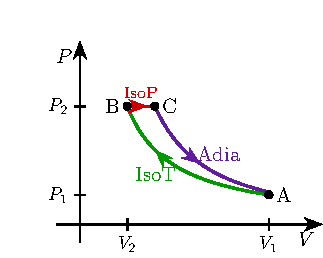
\includegraphics[width=.4\linewidth, valign=t]{E1_watt}
		\hspace*{\fill}
	}{
		\vspace{-30pt}
		\begin{center}
			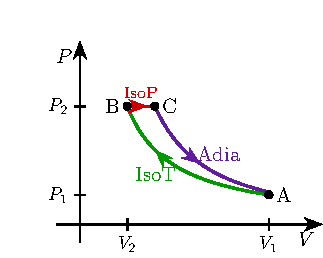
\includegraphics[width=.4\linewidth]{E1_watt}
		\end{center}
	}
}%
\QR{%
	Exprimer et calculer le travail et le transfert thermique pour chacune des
	transformations AB, BC et CA.
}{%
	\begin{center}
		\captionof{table}{Expressions de $U$, $W_p$ et $Q$ pour le gaz parfait
			diatomique}
		\begin{tabularx}{\linewidth}{cYYY}
			\toprule
			\textbf{Transfo.}
			 &
			\textbf{Énergie interne}
			 &
			\textbf{Travail pression}
			 &
			\textbf{Transfert thermique}
			\\
			\midrule
			AB isoT.
			 &
			$\Delta{U}\ind{AB} = 0$
			 &
			$\DS W\ind{AB} = -nRT_A \ln \frac{V_B}{V_A} = \SI{5.1}{kJ}$
			 &
			$\DS Q = -W\ind{AB} = \SI{-5.1}{kJ}$
			\\\addlinespace[0.5em]
			BC isoP.
			 &
			$\Delta{U}\ind{BC} = C_V (T_C - T_B)$
			 &
			$W\ind{BC} = \Delta{U}\ind{BC} - Q\ind{BC} = \SI{-1.7}{kJ}$
			 &
			$Q\ind{BC} = \Delta{H}\ind{BC} = C_P (T_C - T_B) = \SI{5.9}{kJ}$
			\\\addlinespace[1em]
			CA adia.
			 &
			$\Delta{U}\ind{CA} = C_V (T_A - T_C)$
			 &
			$W\ind{CA} = \Delta{U}\ind{CA} = \SI{-4.2}{kJ}$
			 &
			$Q = 0$
			\\
			\bottomrule
		\end{tabularx}
	\end{center}
}%
\QR{%
	De quel type de machine thermique s'agit-il~?
}{%
	$W\ind{cycle} < 0$~: c'est un moteur.
}%

\end{document}
